\def\baselinestretch{1}
%\chapter{RESULTS OF SPECTRAL FITTING AND VARIABILITY STUDIES} \label{chap:results}
\chapter{\MakeUppercase{\ChapterTitleSix}} \label{chap:results}
    \minitoc
    
    \newpage
    \begin{center}
    	\emph{Abstract of chapter \ref{chap:results}}
    \end{center}
    This chapter explores a dataset of Supersoft X-ray Sources (SSS), analyzing their properties and spectral features. We begin by identifying the SSS and plotting their sky positions. An observation journal details the telescopes, instruments, and exposures used to collect data for each source. We then examine the observed count rates of the SSS, both individually and collectively, including a normalized view for better comparison. The best-fit model using the continuum NLTE approach is applied to all SSS, and the resulting fit statistics are presented. Stellar parameters like luminosity, effective temperature, and hydrogen column density are derived for each SSS using this model. We further explore the unfolded spectra obtained after applying the best-fit model, which reveal the intrinsic properties of the SSS after accounting for instrumental effects and absorption. Additionally, the presence of elemental absorption edges within the unfolded spectra is investigated, providing insights into the composition of the material surrounding these SSS objects. Notably, such edges were only found in SSS located in the Milky Way, not the Large Magellanic Cloud. Finally, we perform a detailed timing analysis of the SSS \source\ using lightcurves from the NICER and XMM-Newton observatories. The Lomb-Scargle periodograms are used to identify periodic signals, with notable peaks observed at 0.055 mHz and 0.077 mHz, and their significance is discussed. Sinusoidal fits to the phase-folded lightcurves confirm the presence of periodic modulations, with variability characteristics reported across different energy ranges.
    
    \setcounter{footnote}{\value{footnotecount}}
    
    \newpage
    \section{\MakeUppercase{Source list}} \label{results:source-list}
    	The following table \ref{tab:source-list} lists all the SSS included in the dataset studied in the present work. It provides information on the source name, SSS type, the host galaxy -- either Milky Way (MW) or Large Magellanic Cloud (LMC), right ascension $\alpha$, and declination $\delta$ in degrees.
    	%The list of sources which were studied are listed in table \ref{tab:source-list} below.
    	
    	\renewcommand{\arraystretch}{1.5}
    	\begin{table}[!htb]
    		\centering
    		\caption{List of sources in dataset}
    		\label{tab:source-list}
			\begin{tabular}{cccccc}
			\hline
			\textbf{S. No.} & \textbf{Source} & \textbf{Type} & \textbf{Galaxy} & {$\boldsymbol{\alpha}$ \textbf{(degrees)}} & {$\boldsymbol{\delta}$ \textbf{(degrees)}} \\ \hline
			{1} & {CAL 83} & {XRB} & {LMC} & {85.89233} & {-68.37283} \\
			{2} & {RS Oph} & {SS} & {MW} & {267.55483} & {-6.70791} \\
			{3} & {RX J0019.8+2156} & {CV} & {MW} & {4.95802} & {21.94783} \\
			{4} & {RX J0527.8-6954} & {CV} & {LMC} & {81.95345} & {-69.90247} \\
			{5} & {RX J0925.7-4758} & {XRB} & {MW} & {141.44167} & {-47.97148} \\
			{6} & {V3890 Sgr} & {CN} & {MW} & {277.68037} & {-24.01915} \\ \hline
			\end{tabular}
		\end{table}
		\renewcommand{\arraystretch}{2.2}
		
		The SSS mentioned in table \ref{tab:source-list} are plotted at their respective sky positions using Aladin Sky Atlas\footnote{\url{https://aladin.cds.unistra.fr/}} and presented using figure \ref{fig:sss-sky-position}.

		\begin{figure}[!htb]
			\centering
			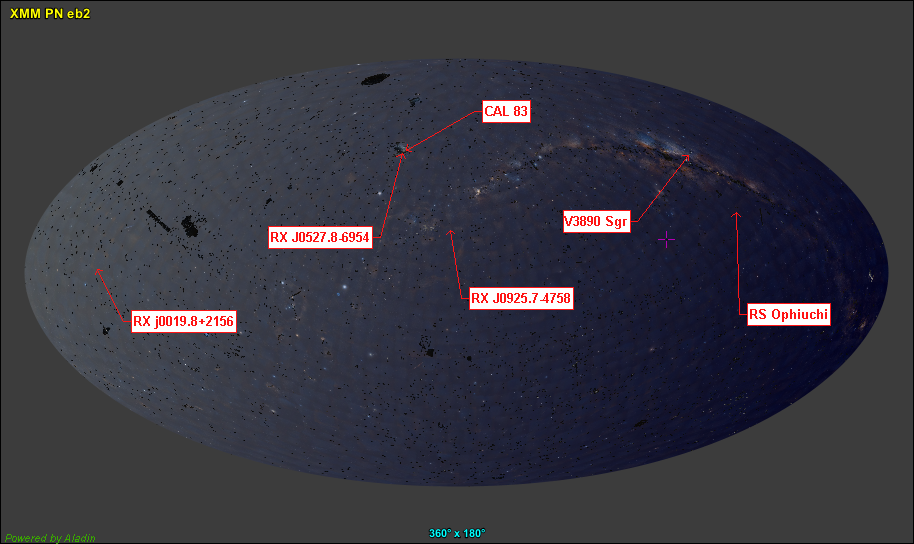
\includegraphics[width=0.8\textwidth]{sss-dataset-positions}
			\caption{Sky positions of SSS chosen for the dataset}
			\label{fig:sss-sky-position}
		\end{figure}

%		\begin{landscape}
%		\begin{figure}[!htb]
%			\centering
%			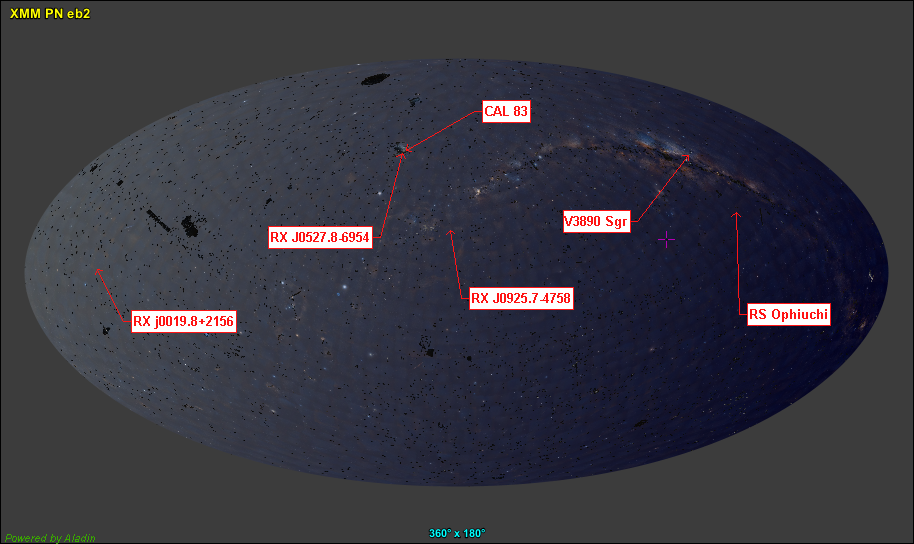
\includegraphics[width=22.0cm]{sss-dataset-positions}
%			\caption{Sky positions of SSS chosen for the dataset}
%			\label{fig:sss-sky-position}
%		\end{figure}
%		\end{landscape}
		
		\begin{landscape}
		\subsection{Journal of Observations}
			The table \ref{tab:sss-obs-list} presents a journal of the SSS observations for each source in the dataset. It includes the source name, the name of the observatory, the instrument used for the observation, the observation ID, the date of observation, the Modified Julian Day (in MJD), exposure time (in kiloseconds), and the observed photon energy range (in keV).
			
			\begin{table}[!htb]
				\centering
	    		\caption{SSS observation journal of dataset}
	    		\label{tab:sss-obs-list}
				\begin{tabular}{cccccccc}
				\hline
				\textbf{Source} & \textbf{Observatory} & \textbf{Instrument} & \textbf{\begin{tabular}[c]{@{}c@{}}Observation\\ (Obs. ID)\end{tabular}} & \textbf{\begin{tabular}[c]{@{}c@{}}Date\\ (yyyy-mm-dd)\end{tabular}} & \textbf{MJD} & \textbf{\begin{tabular}[c]{@{}c@{}}Exposure\\ (ks)\end{tabular}} & \textbf{\begin{tabular}[c]{@{}c@{}}Bandwidth\\ (keV)\end{tabular}} \\ \hline
				{CAL 83} & {XMM-Newton} & {EPIC-pn} & {0506531501} & {2008-08-12} & {54690.62} & {6.9} & {0.2--1.0} \\
				{RS Oph} & {XMM-Newton} & {EPIC-pn} & {0410180501} & {2006-10-09} & {54017.98} & {49.2} & {0.2--2.0} \\
				{RX J0019.8+2156} & {XMM-Newton} & {EPIC-pn} & {0047940101} & {2001-12-31} & {52274.77} & {58.1} & {0.2--0.5} \\
				{RX J0527.8-6954} & {XMM-Newton} & {EPIC-pn} & {0086770101} & {2000-12-19} & {51897.70} & {49.3} & {0.2--0.6} \\
				{RX J0925.7-4758} & {XMM-Newton} & {EPIC-pn} & {0111150101} & {2000-12-16} & {51894.46} & {61.1} & {0.3--1.0} \\
				{V3890 Sgr} & {XMM-Newton} & {EPIC-MOS1} & {0821560201} & {2019-09-14} & {58740.98} & {25.0} & {0.1--2.0} \\ \hline
				\end{tabular}
			\end{table}
		\end{landscape}
			
		\subsection{Supersoft X-ray Count Rates}
			The observed count rates of the sources listed in table \ref{tab:sss-obs-list} are presented in separate sub-figures within figure \ref{result:count-rate:indiv}. Each sub-figure shows the count rate for a specific source across the corresponding energy range specified in table \ref{tab:sss-obs-list}.
			%The count rates of the sources as observed by the respective observatories in table \ref{tab:sss-obs-list} over the respective energy ranges are presented in the sub-figures in \ref{result:count-rate:indiv}.
			\begin{figure}[h!]
				\centering
				\subfloat[CAL 83 \label{count-rate:cal83}]{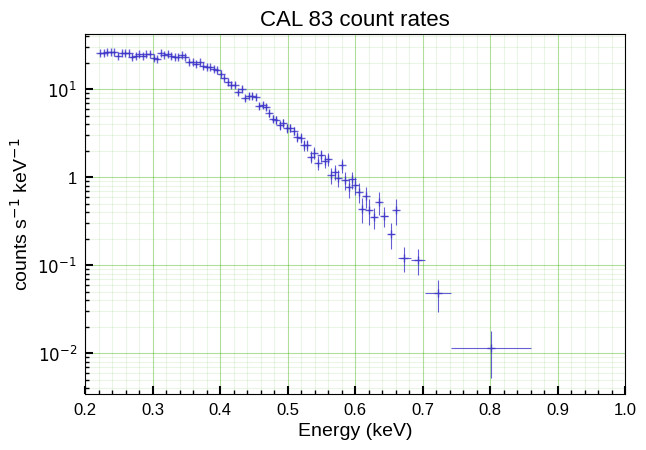
\includegraphics[width=0.45\textwidth]{counts/cal-83-pn_counts}} %\hfill
				\subfloat[RS Oph \label{count-rate:rsoph}]{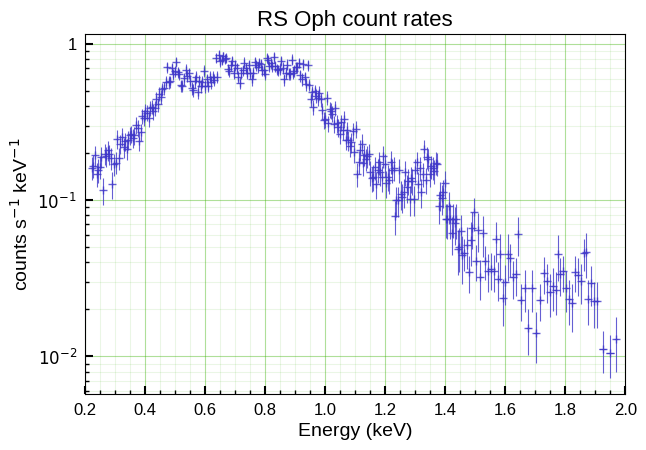
\includegraphics[width=0.45\textwidth]{counts/rs-oph-pn_counts}} %\hfill
				
				\subfloat[RX J0019.8+2156 \label{count-rate:rxj0019}]{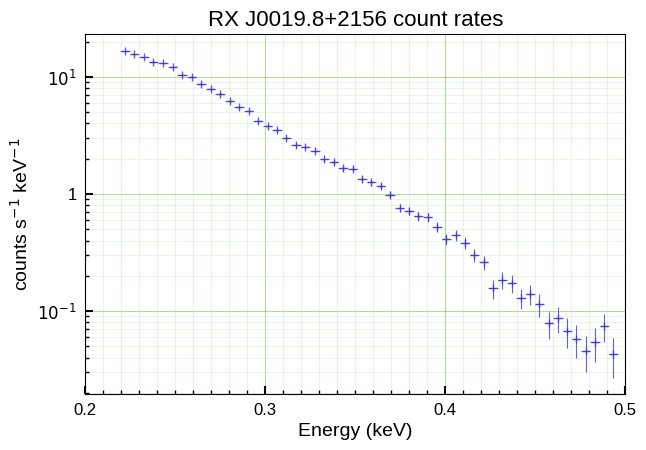
\includegraphics[width=0.45\textwidth]{counts/rx-j0019d8p2156-pn_counts}} %\hfill
				\subfloat[RX J0527.8-6954 \label{count-rate:rxj0527}]{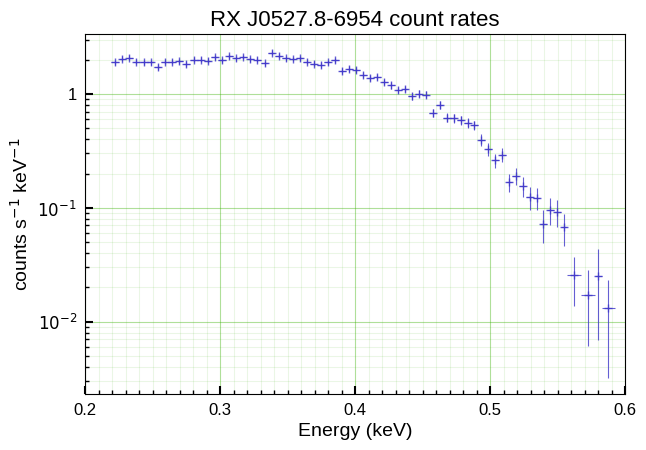
\includegraphics[width=0.45\textwidth]{counts/rx-j0527d8-6954-pn_counts}} %\hfill
				
				\subfloat[RX J0925.7-4758 \label{count-rate:mrvel}]{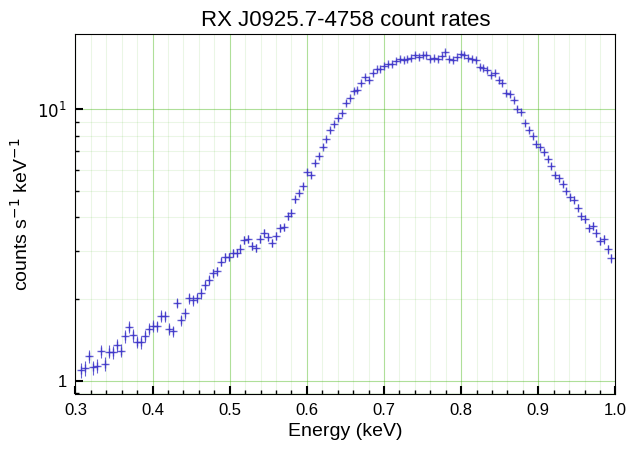
\includegraphics[width=0.45\textwidth]{counts/rx-j0925-4758-pn_counts}} %\hfill
				\subfloat[V3890 Sgr \label{count-rate:v3890}]{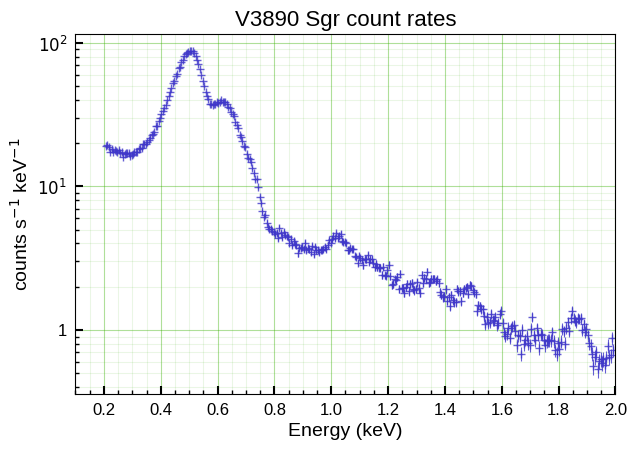
\includegraphics[width=0.45\textwidth]{counts/v3890-sgr-pn_counts}} %\hfill
				\caption{Count rates of individual sources in dataset in SSS regime}
				\label{result:count-rate:indiv}
			\end{figure}
			
			Figure \ref{result:count-rate:all} presents the observed count rates of all sources in the dataset.
			\begin{itemize}
				\item The sub-figure \ref{count-rate:all} presents the raw count rates for each source across the observed energy range, highlighting potential differences in their intrinsic luminosities and/or absorption properties.
				
				\item For a more direct comparison between the source spectra that may have intrinsically different luminosities, the sub-figure \ref{count-rate:all} presents the count rates scaled to a range of 0 to 1 using min-max normalization.%, thereby allowing for a clearer visualization of the spectral shapes across the sources, potentially revealing similarities or differences in their emission profiles.
			\end{itemize}

%    Sub-figure \ref{count-rate:all}: This sub-figure shows the raw count rates for each source across the observed energy range. The varying count rates between the sources highlight potential differences in their intrinsic luminosities and/or absorption properties.
%
%    Sub-figure \ref{count-rate:all-norm}: To facilitate a more direct comparison between the source spectra that may have intrinsically different luminosities, this sub-figure presents the normalized count rates for all sources. The normalization scales the observed counts to a common range of 0 to 1. This allows for a clearer visualization of the spectral shapes across the sources, potentially revealing similarities or differences in their emission line profiles.
			\begin{figure}[h!]
				\centering
				\subfloat[Count rates of all sources \label{count-rate:all}]{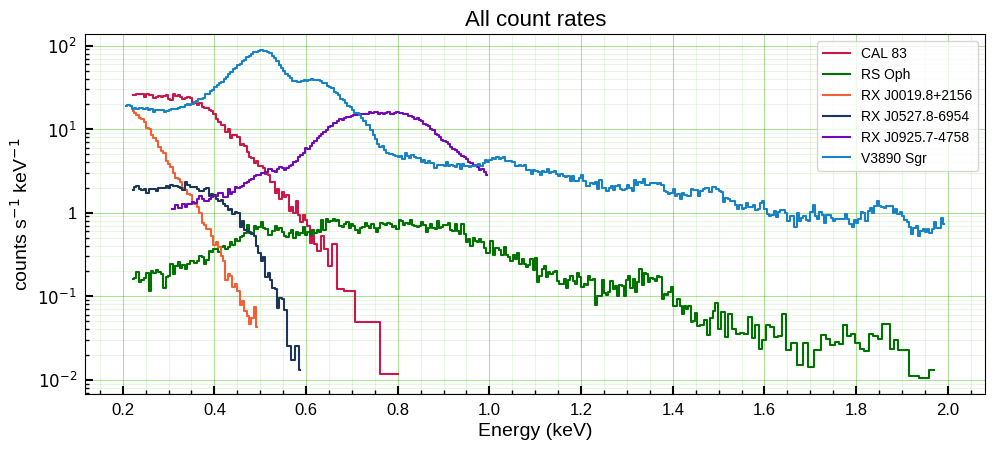
\includegraphics[width=0.9\textwidth]{counts/all_counts}} %\hfill
				
				\subfloat[Normalized count rates of all sources \label{count-rate:all-norm}]{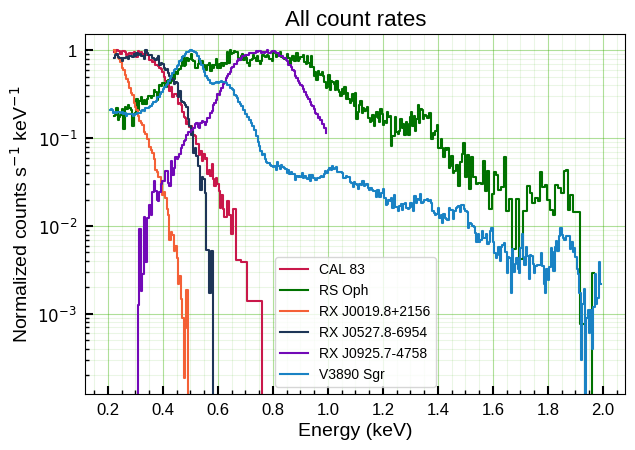
\includegraphics[width=0.9\textwidth]{counts/all_norm-counts}} %\hfill
				\caption{Count rates of all sources in dataset}
				\label{result:count-rate:all}
			\end{figure}
			
	\section{\MakeUppercase{Spectral fitting}} \label{results:spectral}
			
		\subsection{Best-fit Statistics}
			Table \ref{tab:sss-fit-stats} presents the fit statistics for the best-fit model applied to all sources in the dataset using the continuum NLTE model. The table includes the chi-squared value ($\chi^2$), degrees of freedom (d.o.f.), reduced chi-squared value ($\chi^2_\text{reduced}$), and the null hypothesis probability.
			%The fit statistics of the best-fit model for all the sources in the dataset using continuum NLTE model is presented in table \ref{tab:sss-fit-stats}.
			\renewcommand{\arraystretch}{1.8}
			\begin{table}[!htb]
				\centering
				\caption{Fitting statistics for all sources in dataset}
				\label{tab:sss-fit-stats}
				\begin{tabular}{cccc}
					\hline
					\textbf{Source} & {$\boldsymbol{\chi^2}$/\textbf{d.o.f}} & {$\boldsymbol{\chi^2_\text{reduced}}$} & \textbf{\begin{tabular}[c]{@{}c@{}}Null hyp.\\ prob.\end{tabular}} \\ \hline
					{CAL 83} & {${108.0}/{83}$} & {1.30} & {$1.50\times 10^{-2}$} \\
					{RS Oph} & {${189.7}/{135}$} & {1.40} & {$1.35\times 10^{-3}$} \\
					{RX J0019.8+2156} & {${68.3}/{54}$} & {1.26} & {$9.16\times 10^{-2}$} \\
					{RX J0527.8-6954} & {${135.1}/{87}$} & {1.55} & {$7.28\times 10^{-4}$} \\
					{RX J0925.7-4758} & {${183.4}/{131}$} & {1.40} & {$1.73\times 10^{-3}$} \\
					{V3890 Sgr} & {} & {} & {} \\ \hline
				\end{tabular}
			\end{table}
			\renewcommand{\arraystretch}{2.2}
			
		\subsection{Stellar Parameters}
			The stellar parameters for all sources in the dataset, derived using the continuum NLTE model, are presented in table \ref{tab:sss-stellar-params}. The table provides the values of the luminosity ($L_*$), effective temperature ($T_\text{eff}$), and hydrogen column density ($n_H$) for each source, calculated after obtaining the best-fit.
			%The stellar parameters of all the sources in the dataset, computed using continuum NLTE model, is presented in table \ref{tab:sss-stellar-params}.
			\renewcommand{\arraystretch}{1.8}
			\begin{table}[!htb]
				\centering
				\caption{Stellar parameters of all sources from continuum NLTE model}
				\label{tab:sss-stellar-params}
				\begin{tabular}{cccc}
				\hline
				{\textbf{Source}} & {$\boldsymbol{L_*}$ \textbf{(erg s$\boldsymbol{^{-1}}$)}} & {\textbf{$\boldsymbol{T_\text{eff}}$ (kK)}} & {\textbf{$\boldsymbol{n_H}$ ($\boldsymbol{\times 10^{22}}$ cm$\boldsymbol{^{-2}}$)}} \\
				\hline
				{CAL 83} & {$5.9_{-1.4}^{+1.3}\times 10^{38}$} & {$102.9_{-2.1}^{+7.1}$} & {$0.08_{-0.01}^{+0.01}$} \\
				{RS Oph} & {$2.7_{-0.3}^{+5.9}\times 10^{35}$} & {$181.6_{-14.2}^{+18.5}$} & {$0.07_{-0.05}^{+0.10}$} \\
				{RX J0019.8+2156} & {$1.2_{-0.8}^{+1.2}\times 10^{35}$} & {$60.5_{-14.0}^{+10.4}$} & {$0.05_{-0.04}^{+0.76}$} \\
				{RX J0527.8-6954} & {$1.2_{-0.6}^{+0.9}\times 10^{40}$} & {$50.6_{-6.9}^{+3.5}$} & {$0.33_{-0.08}^{+0.01}$} \\
				{RX J0925.7-4758} & {$1.7_{-1.2}^{+1.9}\times 10^{44}$} & {$91.6_{-4.7}^{+8.6}$} & {$1.18_{-0.09}^{+0.09}$} \\
				{V3890 Sgr} & {} & {} & {} \\
				\hline
				\end{tabular}
			\end{table}
			\renewcommand{\arraystretch}{2.2}
			
			In figure \ref{result:L-Teff-SSS}, the calculated values of the luminosities $L_*$ and effective temperature $T_\text{eff}$ for the SSS in our dataset using their respective best-fit models, as presented in table \ref{tab:sss-stellar-params}.
			\begin{figure}[h!]
				\centering
				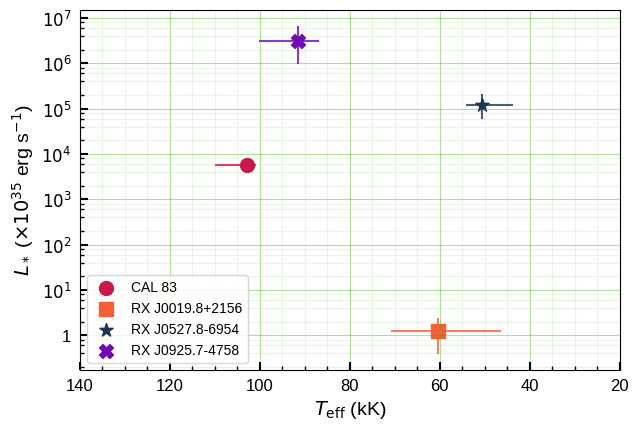
\includegraphics[width=0.8\textwidth]{L-Teff_all-SSS}
				\caption{$L_*$ and $T_\text{eff}$ computed for all SSS in dataset}
				\label{result:L-Teff-SSS}
			\end{figure}
		
		\newpage
		\subsection{Unfolded Spectra from Best-fit Models}
			Unfolded spectra represent the intrinsic spectral energy distribution (SED) of an astronomical object after removing the effects of instrumental response and absorption along the line of sight. The best-fit model accounts for these factors, allowing us to recover the underlying source spectrum. By analyzing the unfolded spectrum, we can identify prominent features such as emission lines and absorption edges. Also, the overall shape of the unfolded spectrum in the continuum region can provide insights into the physical processes responsible for the emission mechanism within the source.
			
			In this section, we present the unfolded spectra obtained after applying the best-fit model derived using the continuum NLTE approach.
		
			\subsubsection*{Unfolded spectrum of CAL 83}
				Figure \ref{result:euf-cal-83} presents the unfolded spectrum of the SSS CAL 83 in the LMC.
				\begin{figure}[h!]
					\centering
					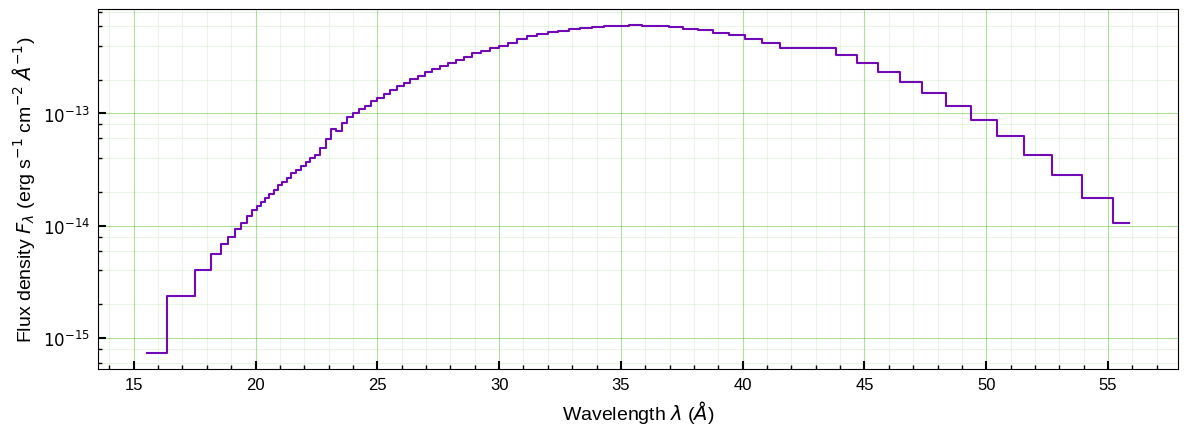
\includegraphics[width=\textwidth]{eufspec/cal-83-pn_eufspec}
					\caption{Unfolded spectrum after model fitting for CAL 83}
					\label{result:euf-cal-83}
				\end{figure}
			
			\newpage
			\subsubsection*{Unfolded spectrum of RS Oph}
				Figure \ref{result:euf-rs-oph} presents the unfolded spectrum of the SSS RS Oph in the MW.
				\begin{figure}[h!]
					\centering
					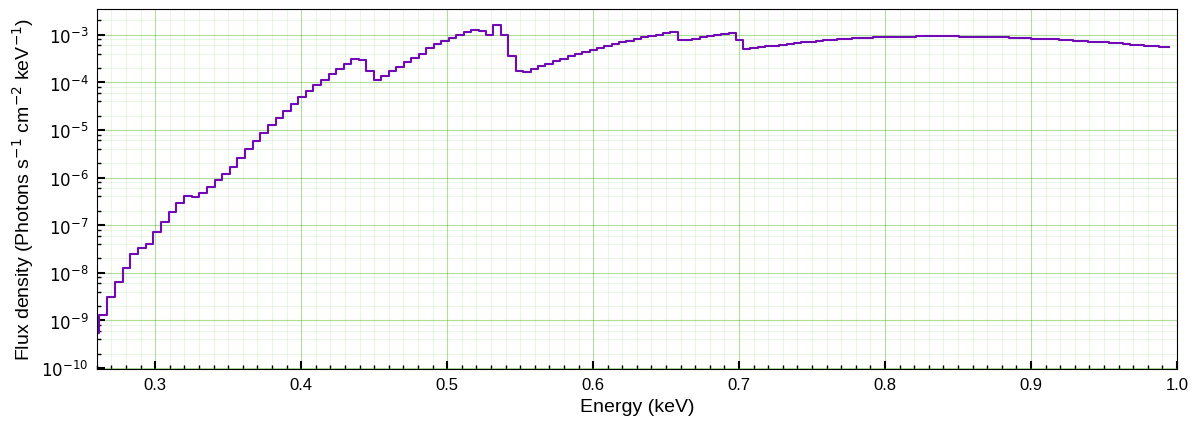
\includegraphics[width=\textwidth]{eufspec/rs-oph-pn_eufspec}
					\caption{Unfolded spectrum after model fitting RS Oph}
					\label{result:euf-rs-oph}
				\end{figure}
			
			\subsubsection*{Unfolded spectrum of RX J0019.8+2156}
				Figure \ref{result:euf-rx-j0019} presents the unfolded spectrum of the SSS RX J0019.8+2156 in the MW.
				\begin{figure}[h!]
					\centering
					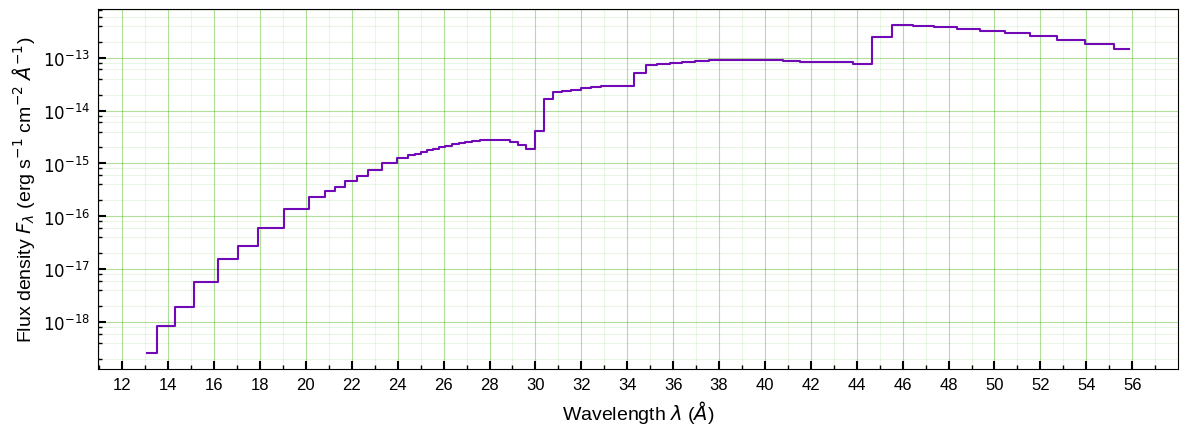
\includegraphics[width=\textwidth]{eufspec/rx-j0019d8p2156-pn_eufspec}
					\caption{Unfolded spectrum after model fitting for RX J0019.8+2156}
					\label{result:euf-rx-j0019}
				\end{figure}
			
			\newpage
			\subsubsection*{Unfolded spectrum of RX J0527.8-6954}
				Figure \ref{result:euf-rx-j0527} presents the unfolded spectrum of the SSS RX J0527.8-6954 in the LMC.
				\begin{figure}[h!]
					\centering
					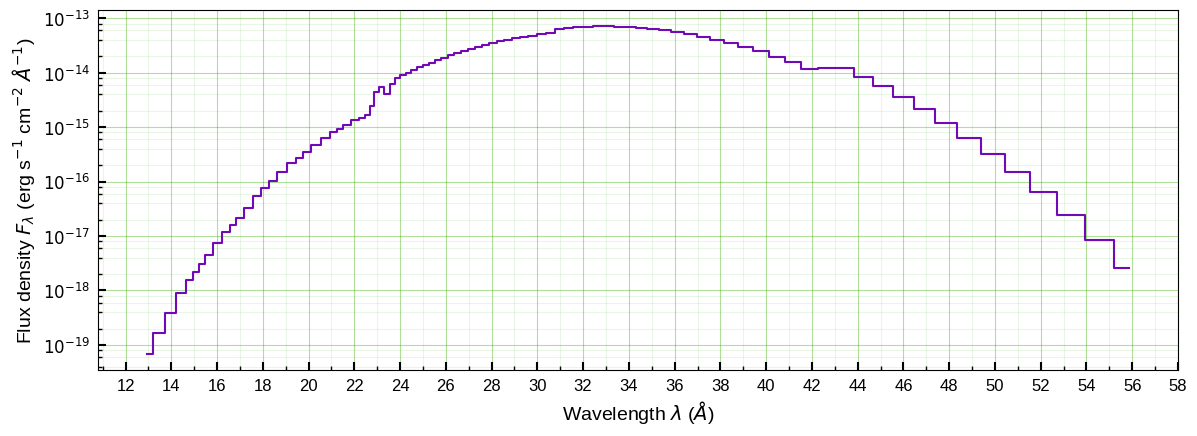
\includegraphics[width=\textwidth]{eufspec/rx-j0527d8-6954-pn_eufspec}
					\caption{Unfolded spectrum after model fitting for RX J0527.8-6954}
					\label{result:euf-rx-j0527}
				\end{figure}
			
			\subsubsection*{Unfolded spectrum of RX J0925.7-4758}
				Figure \ref{result:euf-rx-j0925} presents the unfolded spectrum of the SSS RX J0925.7-4758 in the MW.
				\begin{figure}[h!]
					\centering
					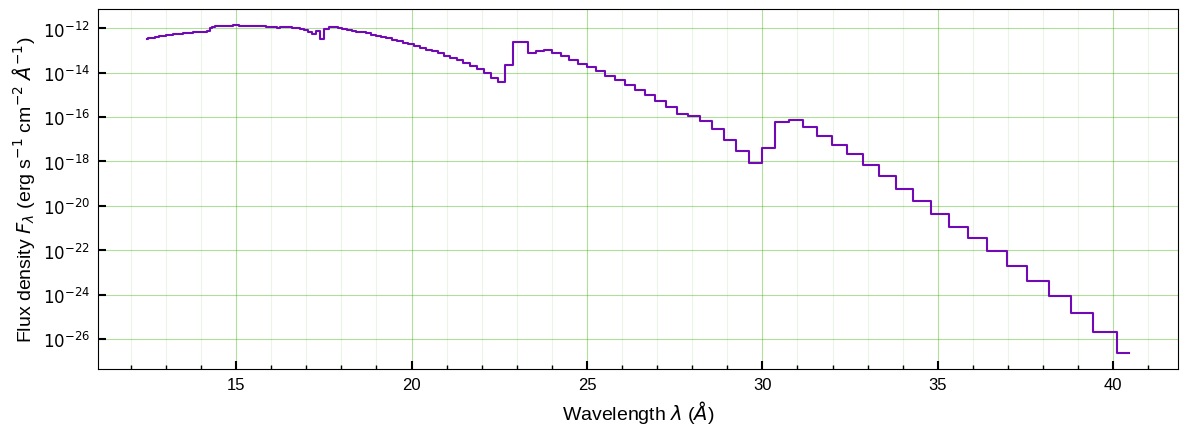
\includegraphics[width=\textwidth]{eufspec/rx-j0925-4758-pn_eufspec}
					\caption{Unfolded spectrum after model fitting for RX J0925.7-4758}
					\label{result:euf-rx-j0925}
				\end{figure}
			
			%\subsection*{Unfolded spectrum of V3890 Sgr}
		
		%\newpage
		\subsection{Presence of Elemental Absorption Edges}
			An absorption edge is a spectral feature which appears as a sharp decrease in intensity at a specific energy in the spectrum. It resembles a step function, with a sudden drop followed by a plateau at a lower intensity level. This occurs when the energy of a photon exactly matches the ionization potential required to remove an electron from a specific energy level (shell) in an atom. The sudden drop happens because a majority of photons at this energy are absorbed. So, while an absorption line represents a \textit{bound-bound transition}, an absorption edge represents a \textit{bound-free transition}.
			
			The presence of various absorption edges provides information about the elemental composition of the absorbing material. The energy at which the edge appears is characteristic of the element responsible for the absorption. In this section, we present the elemental absorption edges identified within the unfolded spectra of specific sources in the dataset. It is noteworthy that identifiable absorption edges were only found within the unfolded spectra of SSS objects located in the Milky Way (MW). No such edges were discernible in the spectra of SSS objects residing in the Large Magellanic Cloud (LMC).
		
			%\subsection*{Absorption lines in CAL 83 spectrum}
			
			\newpage
			\subsubsection*{Absorption edges in RS Oph spectrum}
				\begin{figure}[h!]
					\centering
					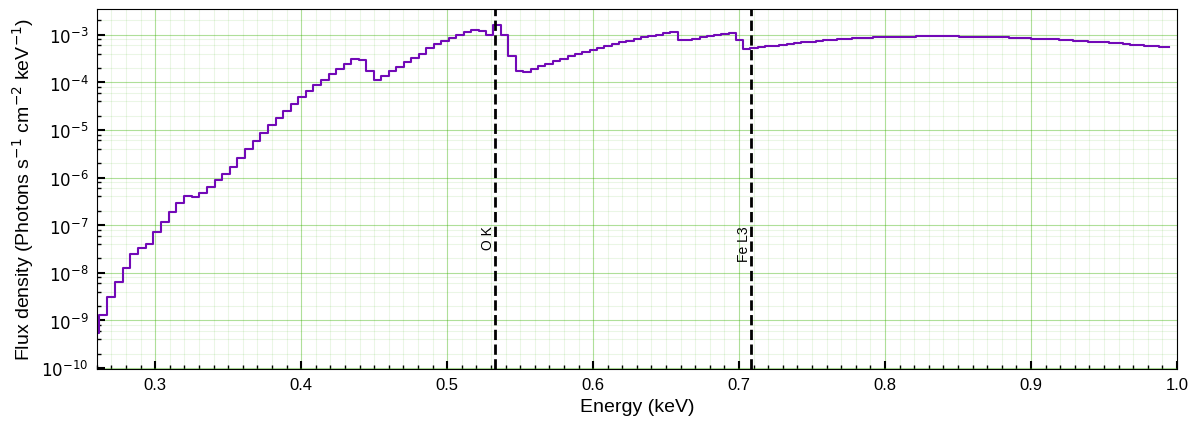
\includegraphics[width=\textwidth]{eufspec/rs-oph-pn_eufspec-keV-edges}
					\caption{Identified absorption edges for RS Oph}
					\label{result:absedge-rs-oph}
				\end{figure}
				
				\renewcommand{\arraystretch}{1.5}
				\begin{table}[!htb]
					\centering
					\caption{Absorption edges identified for RS Oph}
					\label{tab:absedge-rs-oph}
					\begin{tabular}{ccc}
						\hline
						\textbf{Source} & \multicolumn{2}{c}{RS Oph} \\
						\textbf{Observatory} & \multicolumn{2}{c}{XMM-Newton} \\
						\textbf{Obs. ID} & \multicolumn{2}{c}{0410180501} \\
						\textbf{Instrument} & \multicolumn{2}{c}{EPIC-pn} \\
						\textbf{No. of edges identified} & \multicolumn{2}{c}{2} \\
						\textbf{Relative depth} & \multicolumn{2}{c}{0.52 : 1.0} \\
						\hline
						\textbf{Absorption edge} & {O $K$ Edge} & {Fe $L_3$ Edge} \\
						\textbf{Edge energy} & {0.533 keV} & {0.708 keV} \\
						\textbf{Edge depth} & {0.457} & {0.872} \\ \hline
					\end{tabular}
				\end{table}
				\renewcommand{\arraystretch}{2.2}
			
			\newpage
			\subsubsection*{Absorption edges in RX J0019.8+2156 spectrum}
				\begin{figure}[h!]
					\centering
					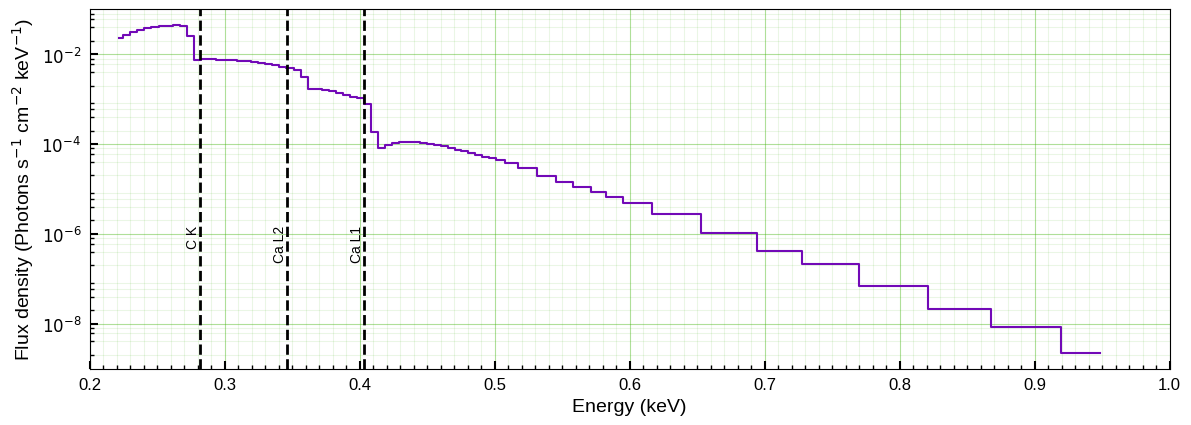
\includegraphics[width=\textwidth]{eufspec/rx-j0019d8p2156-pn_eufspec-keV-edges}
					\caption{Identified absorption edges for RX J0019.8+2156}
					\label{result:absedge-rx-j0019}
				\end{figure}
				
				\renewcommand{\arraystretch}{1.5}
				\begin{table}[!htb]
					\centering
					\caption{Absorption edges identified for RX J0019.8+2156}
					\label{tab:absedge-rx-j0019}
					\begin{tabular}{cccc}
						%\cline{1-3}
						\hline
						\textbf{Source} & \multicolumn{2}{c}{RX J0019.8+2156} & {} \\
						\textbf{Observatory} & \multicolumn{2}{c}{XMM-Newton}& {} \\
						\textbf{Obs. ID} & \multicolumn{2}{c}{0047940101}& {} \\
						\textbf{Instrument} & \multicolumn{2}{c}{EPIC-pn}& {} \\
						\textbf{No. of edges identified} & \multicolumn{2}{c}{3}& {} \\
						\textbf{Relative depth} & \multicolumn{2}{c}{0.93 : 0.03 : 1.0} & {} \\ \hline
						\textbf{Absorption edge} & {C $K$ Edge} & {Ca $L_2$ Edge} & {Ca $L_1$ Edge} \\
						\textbf{Edge energy} & {0.282 keV} & {0.346 keV} & {0.403 keV} \\
						\textbf{Edge depth} & {0.809} & {0.026} & {0.867} \\ \hline
					\end{tabular}
				\end{table}
				\renewcommand{\arraystretch}{2.2}
			
			%\subsection*{Absorption lines in RX J0527.8-6954 spectrum}
			
			\newpage
			\subsubsection*{Absorption edges in RX J0925.7-4758 spectrum}
				\begin{figure}[h!]
					\centering
					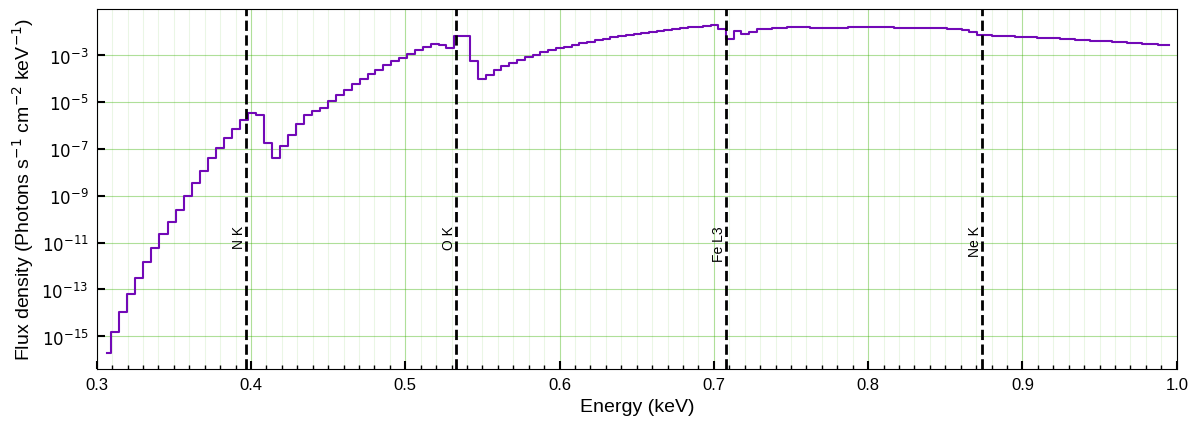
\includegraphics[width=\textwidth]{eufspec/rx-j0925-4758-pn_eufspec-keV-edges}
					\caption{Identified absorption edges from RX J0925.7-4758 spectrum}
					\label{result:absedge-rx-j0925}
				\end{figure}
				
				\renewcommand{\arraystretch}{1.5}
				\begin{table}[!htb]
					\centering
					\caption{Absorption edges identified for RX J0925.7-4758}
					\label{tab:absedge-rx-j0925}
					\begin{tabular}{ccccc}
						%\cline{1-3}
						\hline
						\textbf{Source} & \multicolumn{2}{c}{RX J0925.7-4758} & {} & {} \\
						\textbf{Observatory} & \multicolumn{2}{c}{XMM-Newton} & {} & {} \\
						\textbf{Obs. ID} & \multicolumn{2}{c}{0111150101} & {} & {} \\
						\textbf{Instrument} & \multicolumn{2}{c}{EPIC-pn} & {} & {} \\
						\textbf{No. of edges identified} & \multicolumn{2}{c}{4} & {} & {} \\
						\textbf{Relative depth} & \multicolumn{2}{c}{1.0 : 0.03 : 0.01 : 0.04} & {} & {} \\ \hline
						\textbf{Absorption edge} & {N $K$ Edge} & {O $K$ Edge} & {Fe $L_3$ Edge} & {Ne $K$ Edge} \\
						\textbf{Edge energy} & {0.397 keV} & {0.533 keV} & {0.708 keV} & {0.874 keV} \\
						\textbf{Edge depth} & {5.215} & {0.132} & {0.033} & {0.211} \\ \hline
					\end{tabular}
				\end{table}
				\renewcommand{\arraystretch}{2.2}
			
			%\subsection*{Absorption edges in V3890 Sgr spectrum}
	    
	%    \section{\MakeUppercase{Spectral Line Identification}}
	%    
	%    \section{\MakeUppercase{XMM-Newton RGS Spectral Fit}}
	%    The best fit model, i.e. M11, contains two different additive components that simulate optically thin plasma. One of them, i.e. \texttt{apec} uses line lists from the AtomDB database, while the other, i.e. \texttt{mekal} which is based on calculations by Mewe, Kaastra and Liedahl \cite{meka,liedahl}. The latter could indicate the presence of a hot corona. The presence of the \texttt{rauch} model component in the best fit model suggests a substantial contribution due to an NLTE stellar atmosphere. The model also consists of the \texttt{swind1} component, which simulates the presence of a stellar wind component along the line-of-sight. The presence of all the above model components vindicates our hypothesis of the inclusion of non-steady states, NLTE and stellar winds in the radiative processes in X-ray binary systems such as those of RX J0925.7-4758.
	%    
	%    \section{\MakeUppercase{P Cygni Profiling}}
	
	\newpage
	\section{\MakeUppercase{Variability study of \source}} \label{results:variability}
		In this section, we present the results obtained from a detailed timing analysis of the NICER lightcurves for the source RX J0925.7-4758. The analysis was conducted using the \textit{Lomb-Scargle periodogram}, a well-established method for identifying periodic signals in unevenly sampled time-series data.
	
		\subsection{Observed NICER and XMM-Newton Lightcurves}
			\begin{figure}[h!]
				\centering
				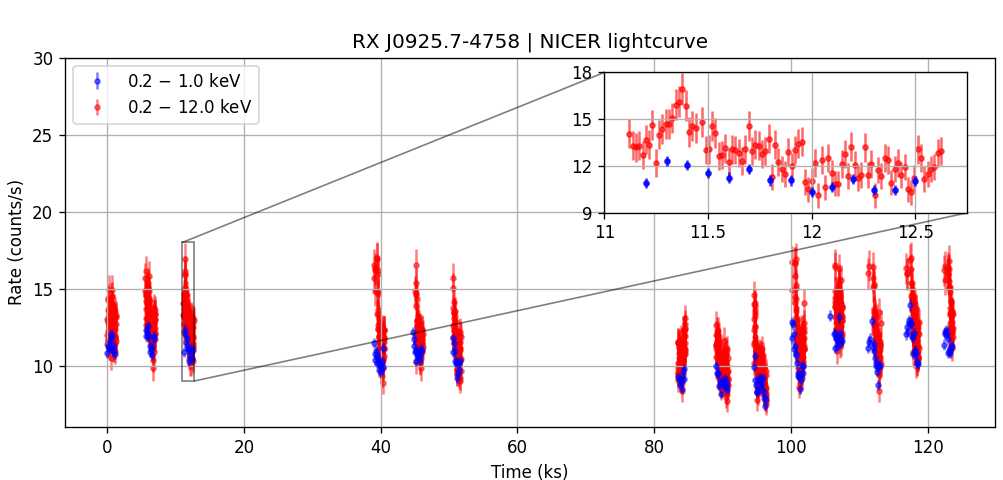
\includegraphics[width=\textwidth]{timing/rx-j0925_lc-bothbands-inset}
				\caption{NICER lightcurves of \source\ using 16 s time bins}
				\label{result:lc-mrvel-nicer}
			\end{figure}
			
			\begin{figure}[h!]
				\centering
				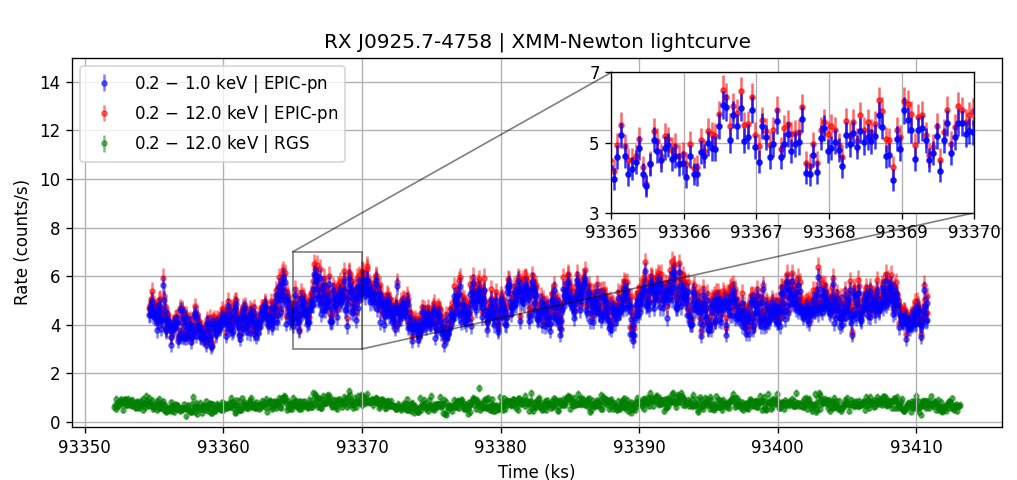
\includegraphics[width=\textwidth]{timing/rx-j0925_0111150101_lc-allbands-inset}
				\caption{XMM-Newton lightcurves of \source\ using 50 s time bins}
				\label{result:lc-mrvel-xmm}
			\end{figure}
			
			The lightcurves of the SSS \source\ as observed by the observatories NICER and XMM-Newton are presented here. For the NICER observations, the lightcurves are extracted by combining timing data from all three observations mentioned in table \ref{tab:obs-journal} using time bins of 16 s, and for XMM-Newton observations, the lightcurves are extracted from the timing data in observation ID 0111150101 using time bins of 50 s. Figures \ref{result:lc-mrvel-nicer} and \ref{result:lc-mrvel-xmm} respectively display the lightcurves extracted from NICER and XMM-Newton data over 0.2--1.0 keV and 0.2--12.0 keV photon energy ranges (the former is the range analysed in the multi-observatory spectral analysis of \source\ described in chapter \ref{chap:multi-obs}, whereas the latter is the full range for SSS).
			
			As expected, the count rates for the lightcurve extracted over the full SSS photon energy range is higher than that for the 0.2--1.0 keV range. This can be seen in the insets in both figures \ref{result:lc-mrvel-nicer} and \ref{result:lc-mrvel-xmm} for the chosen sub-intervals of observations. In figure \ref{result:lc-mrvel-xmm}, we can also see that the count rates of the RGS observations are much smaller than the corresponding EPIC-pn observations.
			
		\subsection{Timing Analysis of NICER Lightcurves}		
			We present here the results of the timing analysis by applying the Lomb-Scargle periodogram on the NICER lightcurves of \source. The use of this technique allows us to extract reliable periodic information from the NICER observations, overcoming potential issues related to gaps in data acquisition or variable observational cadence.
			
			The lightcurves were examined in two distinct photon energy ranges: 0.2--1.0 keV and 0.2--12.0 keV. The former range aligns with the energy band used in the earlier spectral analysis of the source, providing a direct comparison of the timing characteristics within the same spectral window. The latter range encompasses the full energy band for SSS, thereby offering a comprehensive view of the timing behaviour across the entire spectrum accessible to NICER.
			
			\subsubsection{Lomb-Scargle Periodograms}
				\begin{figure}[h!]
					\centering
					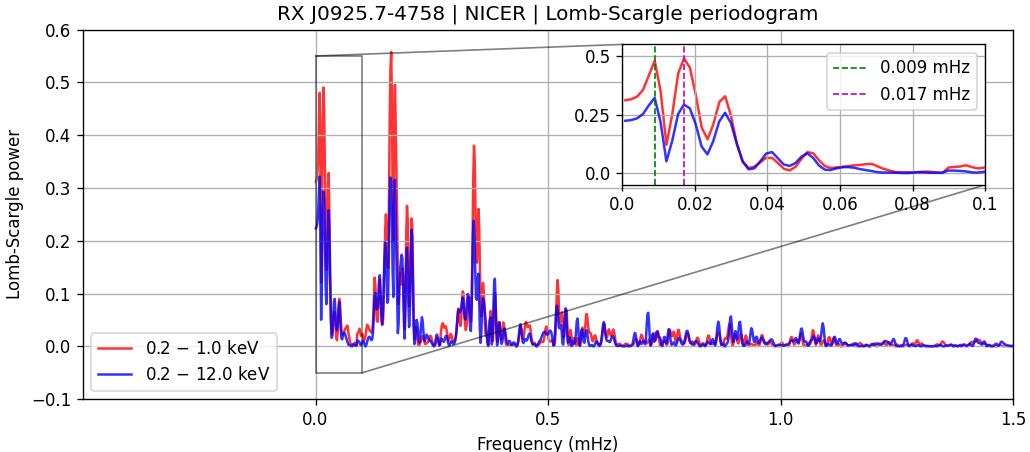
\includegraphics[width=\textwidth]{timing/rx-j0925_nicer-ls_bothbands-inset}
					\caption{Lomb-Scargle periodogram of NICER lightcurves}
					\label{result:ls-mrvel-nicer}
				\end{figure}
				The Lomb-Scargle periodograms were calculated for the lightcurves across both photon energy ranges. The resulting periodograms are depicted in figure \ref{result:ls-mrvel-nicer}. Upon examination of the inset, we observe closely spaced peaks at frequencies of 0.009 mHz and 0.017 mHz, which appear consistently in both energy ranges. These frequencies correspond to periods of 112.3 ks and 58.8 ks respectively, with the latter possibly being a harmonic. So we may consider 0.009 mHz to be an intrinsic variation in the source signal.
				
				Additionally, peaks are identified at higher frequencies, specifically at 0.163 mHz, 0.341 mHz, and 0.521 mHz. However, it is important to note that these higher frequency peaks are attributed to the observational cadence of the NICER XTI, i.e. they correspond to the NICER observation windows, which are separated by approximately 6144 seconds, and represent harmonics of this fundamental period. These peaks do not necessarily indicate intrinsic periodicity in the source but rather reflect the instrumental observational pattern.
			
			\subsubsection{Best-Fit Sinusoids for 0.2--1.0 keV Lightcurve}
				\paragraph{Fitting with phase-folded lightcurve:}
				\begin{figure}[h!]
					\centering
					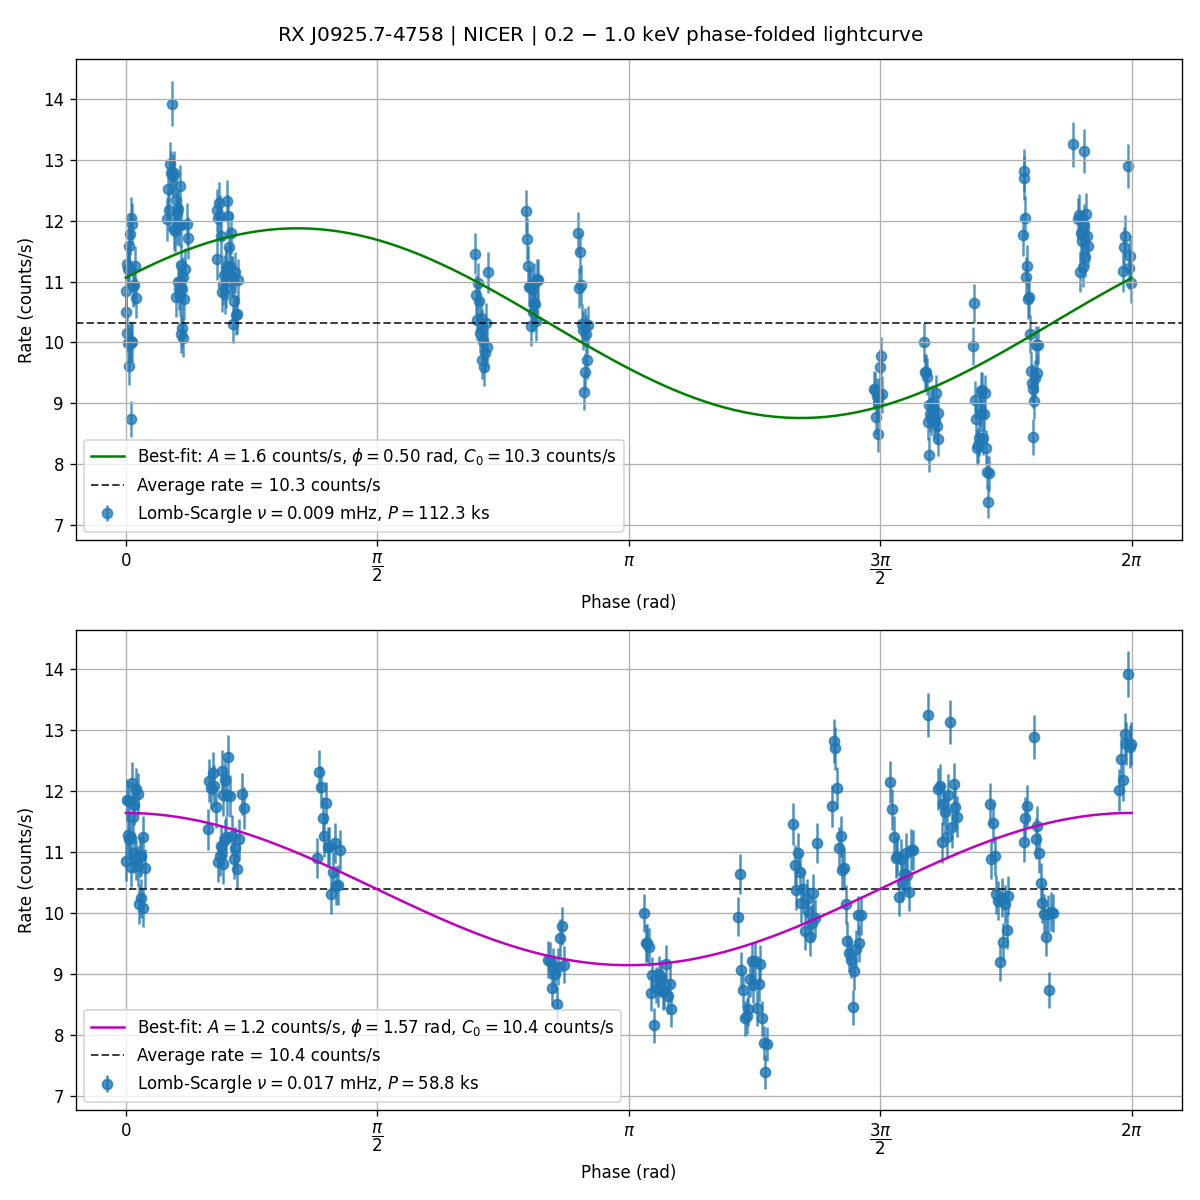
\includegraphics[width=\textwidth]{timing/rx-j0925_nicer-lc_200-1000_phasefold-bestfit}
					\caption{Phase-folded NICER lightcurve over 0.2--1.0 keV with best-fit sinusoids}
					\label{result:lc-phase-fold-mrvel-nicer:200-1000-bestfit}
				\end{figure}
				Utilising the frequencies corresponding to the peak power densities at 0.009 mHz and 0.017 mHz, we performed sinusoidal fits to the NICER lightcurve data. The resulting phase-folded lightcurve, spanning a single cycle from 0 to $2\pi$ radians, is presented in figure \ref{result:lc-phase-fold-mrvel-nicer:200-1000-bestfit} for the photon energy range of 0.2--1.0 keV. This phase-folded representation provides a clearer view of the periodic variations in the lightcurve and highlights the sinusoidal nature of the observed modulation within this specific energy band. Additionally, the best-fit sinusoids are overlaid on top of the phase-folded data, illustrating the close agreement between the model and the observed lightcurve, thereby affirming the periodicity at these frequencies.
				
				\paragraph{Fitting with complete lightcurve:}
				\begin{figure}[h!]
					\centering
					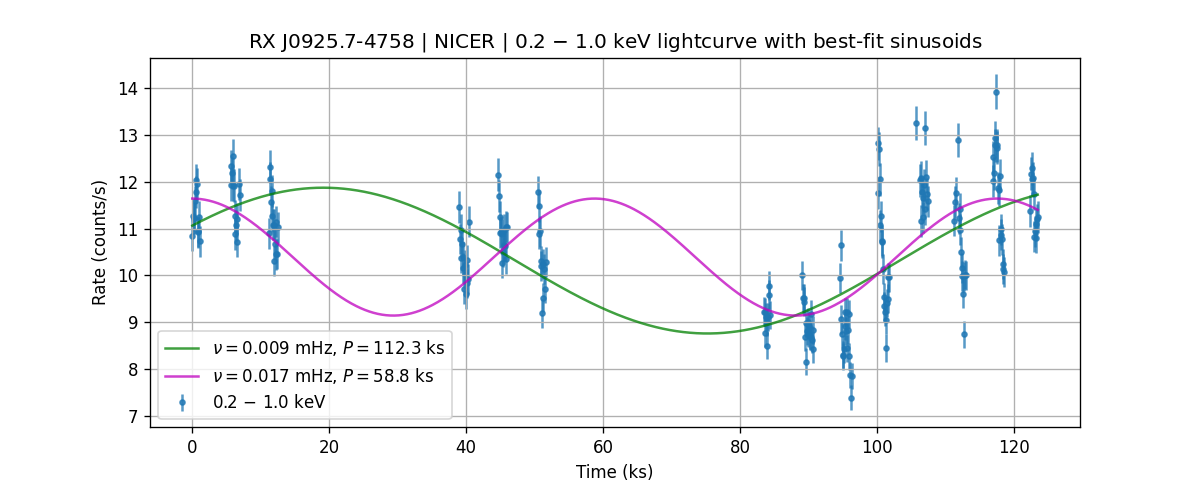
\includegraphics[width=\textwidth]{timing/rx-j0925_nicer-lc_200-1000_bestfit}
					\caption{NICER lightcurve over 0.2--1.0 keV with best-fit sinusoids}
					\label{result:lc-mrvel-nicer:200-1000-bestfit}
				\end{figure}
				To further illustrate the periodic nature of the emission from RX J0925.7-4758, the best-fit sinusoids have also been overlaid on the complete NICER lightcurve, as shown in figure \ref{result:lc-mrvel-nicer:200-1000-bestfit}. This figure provides a comprehensive view of the model's fit over the entire observation period, rather than just a phase-folded representation. By overlaying the best-fit sinusoids directly on the unmodified lightcurve, we can visually assess the alignment of the observed data points with the fitted model across different time intervals.
				
				The strong correspondence between the sinusoidal fits and the actual lightcurve further corroborates the presence of these low-frequency modulations and supports the reliability of the Lomb-Scargle periodogram results in characterising the periodic variability of \source.
				
			\subsubsection{Best-Fit Sinusoids for 0.2--12.0 keV Lightcurve}
				\paragraph{Fitting with phase-folded lightcurve:}				
				\begin{figure}[h!]
					\centering
					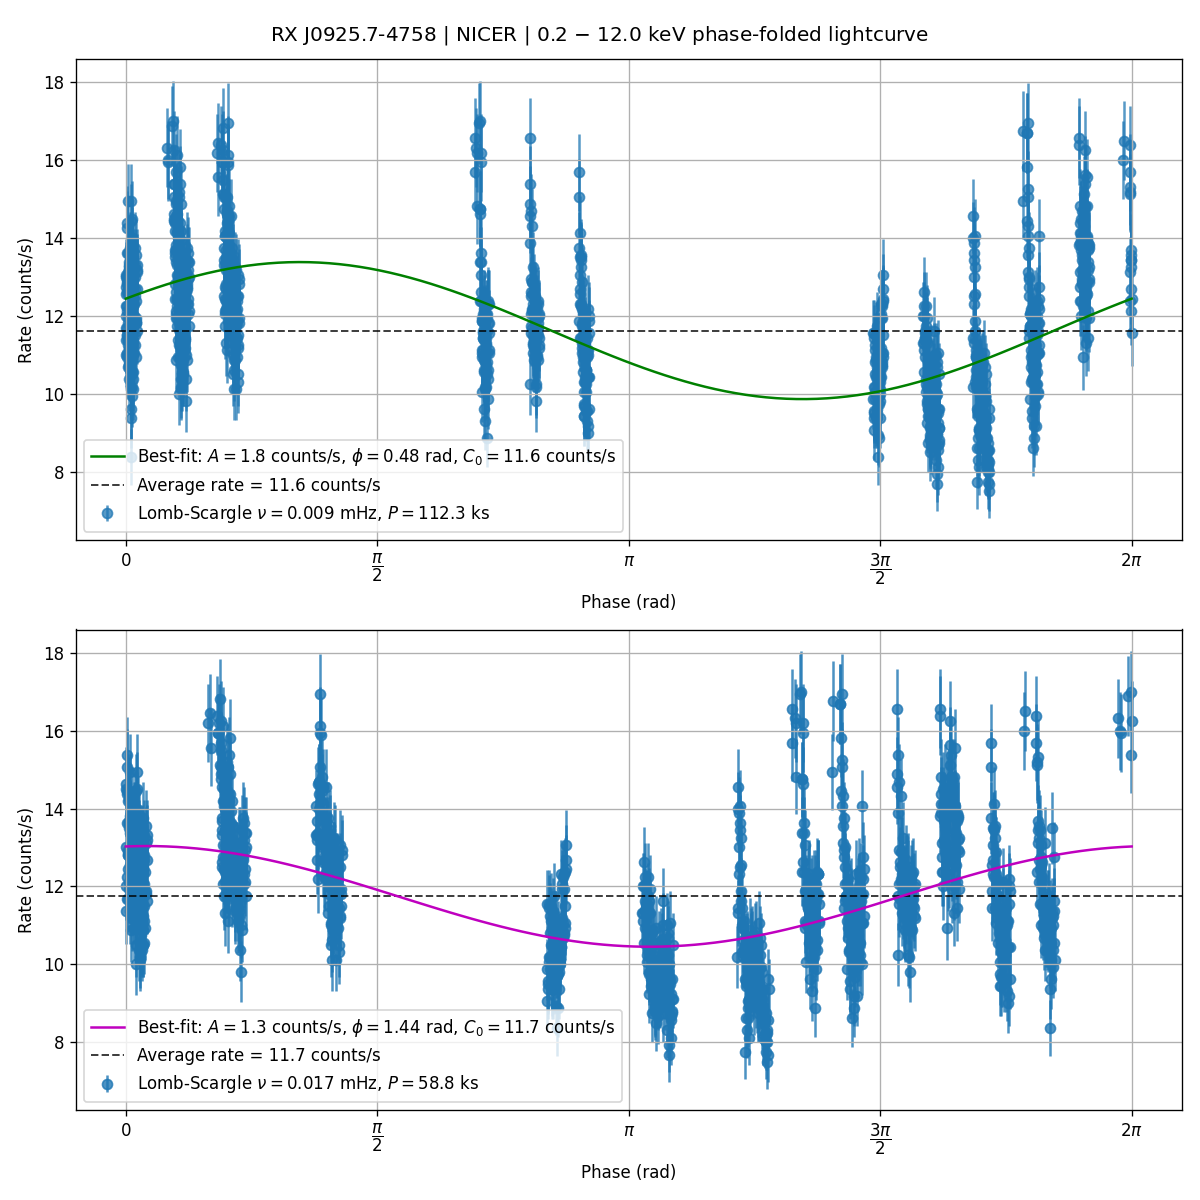
\includegraphics[width=\textwidth]{timing/rx-j0925_nicer-lc_200-12000_phasefold-bestfit}
					\caption{Phase-folded NICER lightcurve over 0.2--12.0 keV with best-fit sinusoids}
					\label{result:lc-phase-fold-mrvel-nicer:200-12000-bestfit}
				\end{figure}
				For the broader 0.2--12.0 keV photon energy range, sinusoidal fits were also applied using the identified frequencies of 0.009 mHz and 0.017 mHz. The resulting phase-folded lightcurve, spanning one full cycle from 0 to $2\pi$ radians, is displayed in figure \ref{result:lc-phase-fold-mrvel-nicer:200-12000-bestfit}. The phase-folded data, with the best-fit sinusoids overlaid, demonstrate periodic modulations consistent with those observed in the narrower 0.2--1.0 keV range. %As highlighted by the best-fit parameters reported in table \ref{tab:timing-mrvel}, both energy ranges exhibit similar variability characteristics, indicating stable periodicities across the SSS spectrum.
				
				\paragraph{Fitting with complete lightcurve:}
				\begin{figure}[h!]
					\centering
					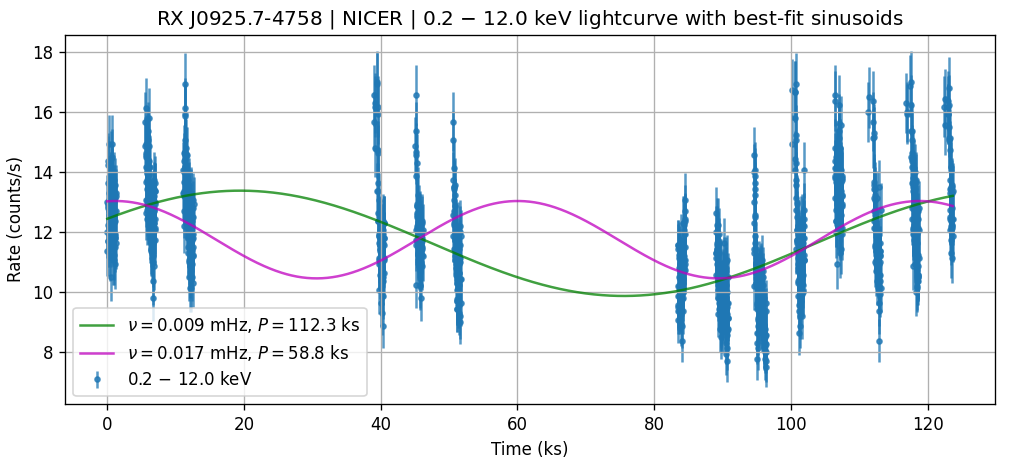
\includegraphics[width=\textwidth]{timing/rx-j0925_nicer-lc_200-12000_bestfit}
					\caption{NICER lightcurve over 0.2--12.0 keV with best-fit sinusoids}
					\label{result:lc-mrvel-nicer:200-12000-bestfit}
				\end{figure}
				For the 0.2--12.0 keV photon energy range, the best-fit sinusoids were similarly overlaid on the complete NICER lightcurve, as depicted in figure \ref{result:lc-mrvel-nicer:200-12000-bestfit}. This visualisation provides an overall view of the model's fit across the entire dataset, enabling a direct comparison of the modelled periodic variations with the observed lightcurve over extended periods. The alignment between the best-fit sinusoids and the actual data points consistently supports the presence of low-frequency modulations in this broader energy band.
				
				
		\subsection{Timing Analysis of XMM-Newton Lightcurves}
			In addition to the NICER observations, we conducted a timing analysis using lightcurves obtained from the EPIC-pn and RGS instruments onboard the XMM-Newton observatory. Similar to the NICER data, we applied the Lomb-Scargle periodogram to these lightcurves to detect and characterise periodic signals. The analysis was performed for the same photon energy ranges: 0.2--1.0 keV and 0.2--12.0 keV. Notably, the XMM-Newton observations were conducted over a continuous observation window of approximately 55 ks, reducing the impact of gaps in data acquisition and improving the reliability of the periodicity detection.
			
			\subsubsection{Lomb-Scargle Periodograms}
				\begin{figure}[h!]
					\centering
					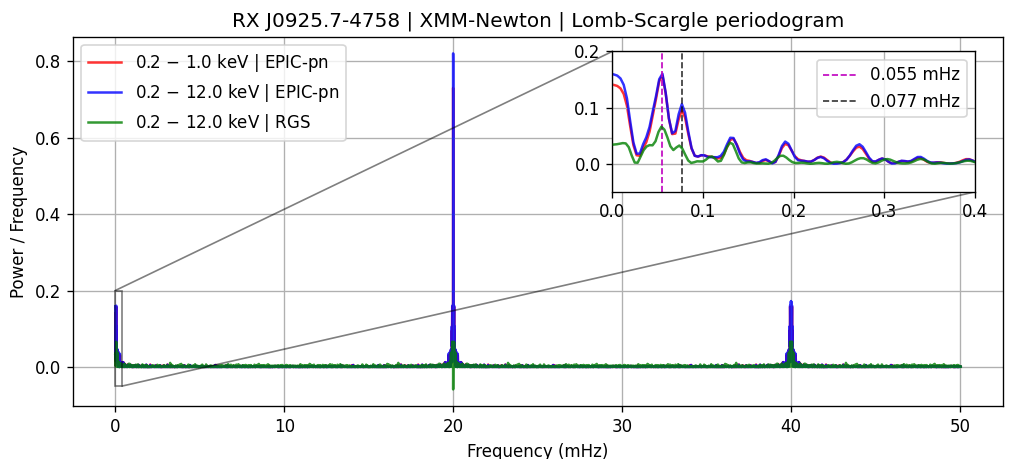
\includegraphics[width=\textwidth]{timing/rx-j0925_0111150101_xmm-ls_allbands-inset}
					\caption{Lomb-Scargle periodogram of XMM-Newton lightcurves}
					\label{result:ls-mrvel-xmm}
				\end{figure}
				The Lomb-Scargle periodograms were also calculated for the lightcurves obtained from the EPIC-pn and RGS instruments of the XMM-Newton observatory, analysed across the same photon energy ranges of 0.2--1.0 keV and 0.2--12.0 keV. The resulting periodograms are depicted in figure \ref{result:ls-mrvel-xmm}. As it can be noticed in the inset, the periodograms reveal two prominent peaks at 0.055 mHz and 0.077 mHz, consistently appearing in both energy ranges and for both instruments. These frequencies correspond to periods of approximately 18.1 ks and 13.1 ks, respectively, indicating potential intrinsic periodicities in the source RX J0925.7-4758. The peaks observed with the RGS instrument are less pronounced, likely due to the lower flux levels in the RGS data compared to EPIC-pn.
				
				In addition, higher frequency peaks are observed at 20 mHz and 40 mHz. However, these are attributed to harmonics introduced by the binning of the lightcurve data, with the 20 mHz peak corresponding to a time period of 50 seconds, which matches our chosen bin size. Therefore, these high-frequency peaks are artefacts of the temporal resolution rather than indicative of intrinsic variability in the source.
			
			\subsubsection{Best-Fit Sinusoids for 0.2--1.0 keV EPIC-pn Lightcurve}
				\paragraph{Fitting with phase-folded lightcurve:}
				For the 0.2--1.0 keV photon energy range obtained from the EPIC-pn instrument of the XMM-Newton observatory, sinusoidal fits were performed using the frequencies with peak power densities observed at 0.055 mHz and 0.077 mHz. The resulting phase-folded lightcurve, covering a single cycle from 0 to $2\pi$ radians, is shown in figure \ref{result:lc-phase-fold-mrvel-xmm:200-1000-bestfit}. The best-fit sinusoids are overlaid on the phase-folded data, demonstrating a strong correspondence between the model and the observed lightcurve.
				\newpage
				\begin{figure}[h!]
					\centering
					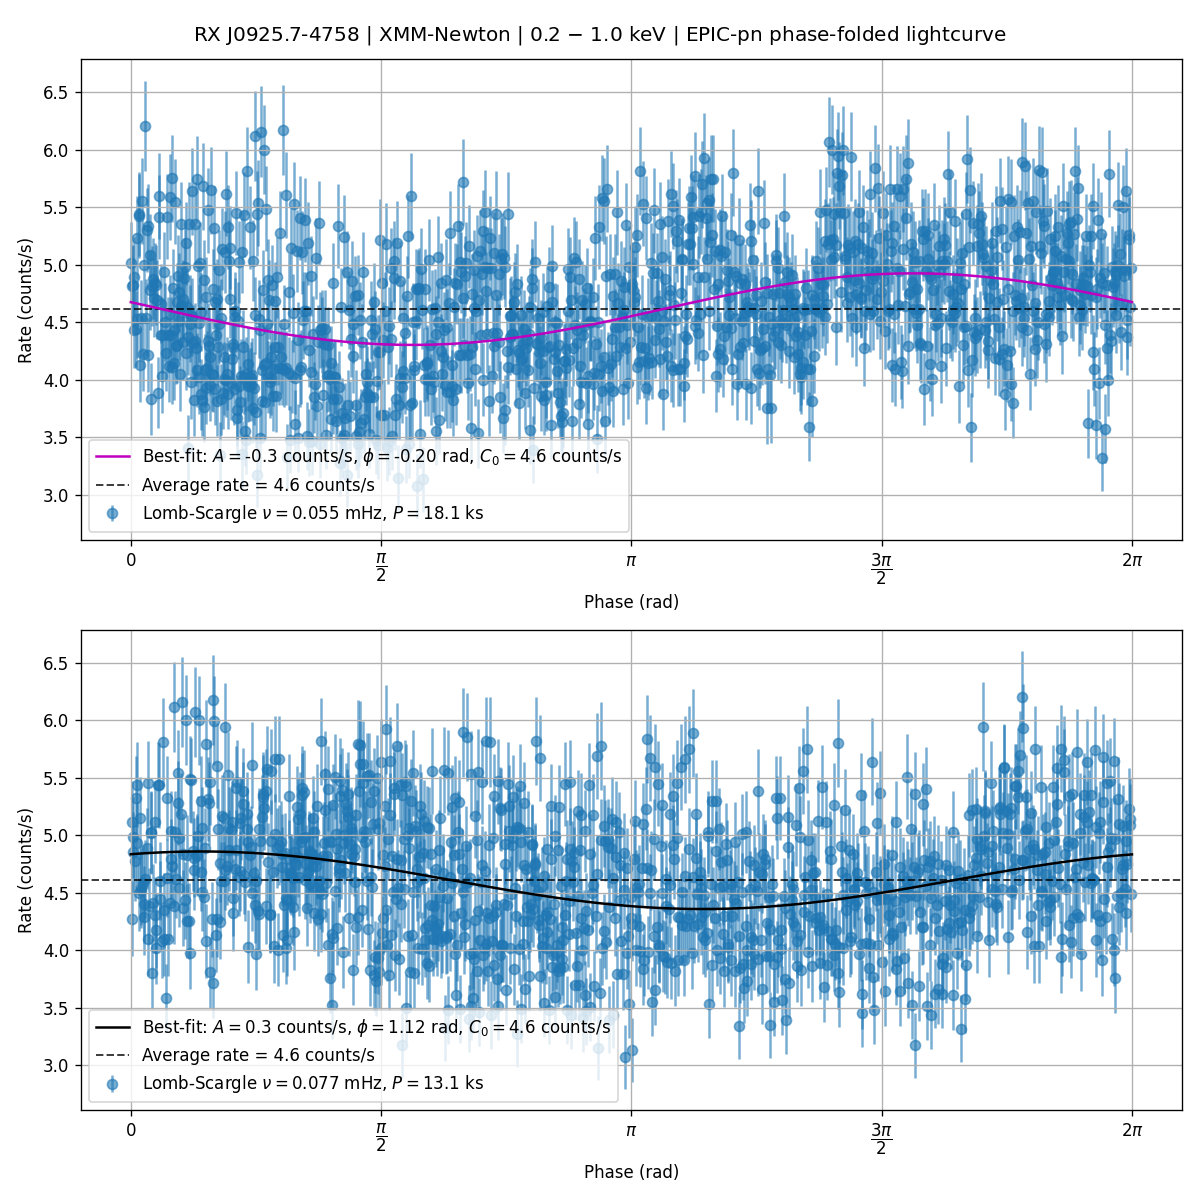
\includegraphics[width=\textwidth]{timing/rx-j0925_0111150101_xmm-lc_200-1000_phasefold-bestfit}
					\caption{Phase-folded XMM-Newton EPIC-pn lightcurve over 0.2--1.0 keV with best-fit sinusoids}
					\label{result:lc-phase-fold-mrvel-xmm:200-1000-bestfit}
				\end{figure}
				
				\paragraph{Fitting with complete lightcurve:}
				\begin{figure}[h!]
					\centering
					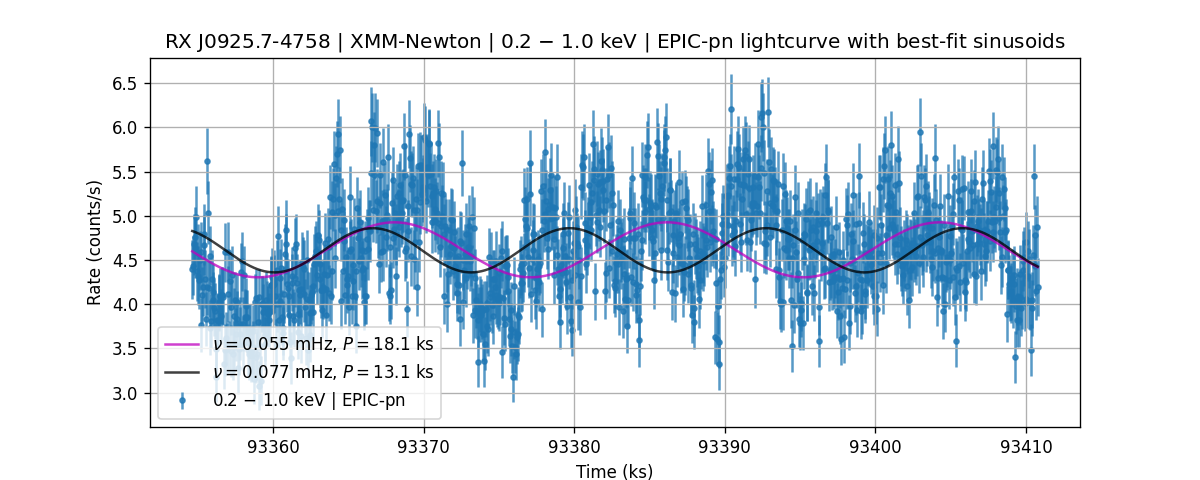
\includegraphics[width=\textwidth]{timing/rx-j0925_0111150101_xmm-lc_200-1000_bestfit}
					\caption{XMM-Newton EPIC-pn lightcurve over 0.2--1.0 keV with best-fit sinusoids}
					\label{result:lc-mrvel-xmm:200-1000-bestfit}
				\end{figure}
				The best-fit sinusoids have also been overlaid on the complete lightcurve for the 0.2--1.0 keV photon energy range using the EPIC-pn instrument of the XMM-Newton observatory. From figure \ref{result:lc-mrvel-xmm:200-1000-bestfit}, we can perform a visual assessment of the agreement between the observed data points with the fitted sinusoid models.
				
			\subsubsection{Best-Fit Sinusoids for 0.2--12.0 keV EPIC-pn Lightcurve}
				\paragraph{Fitting with phase-folded lightcurve:}
				\begin{figure}[h!]
					\centering
					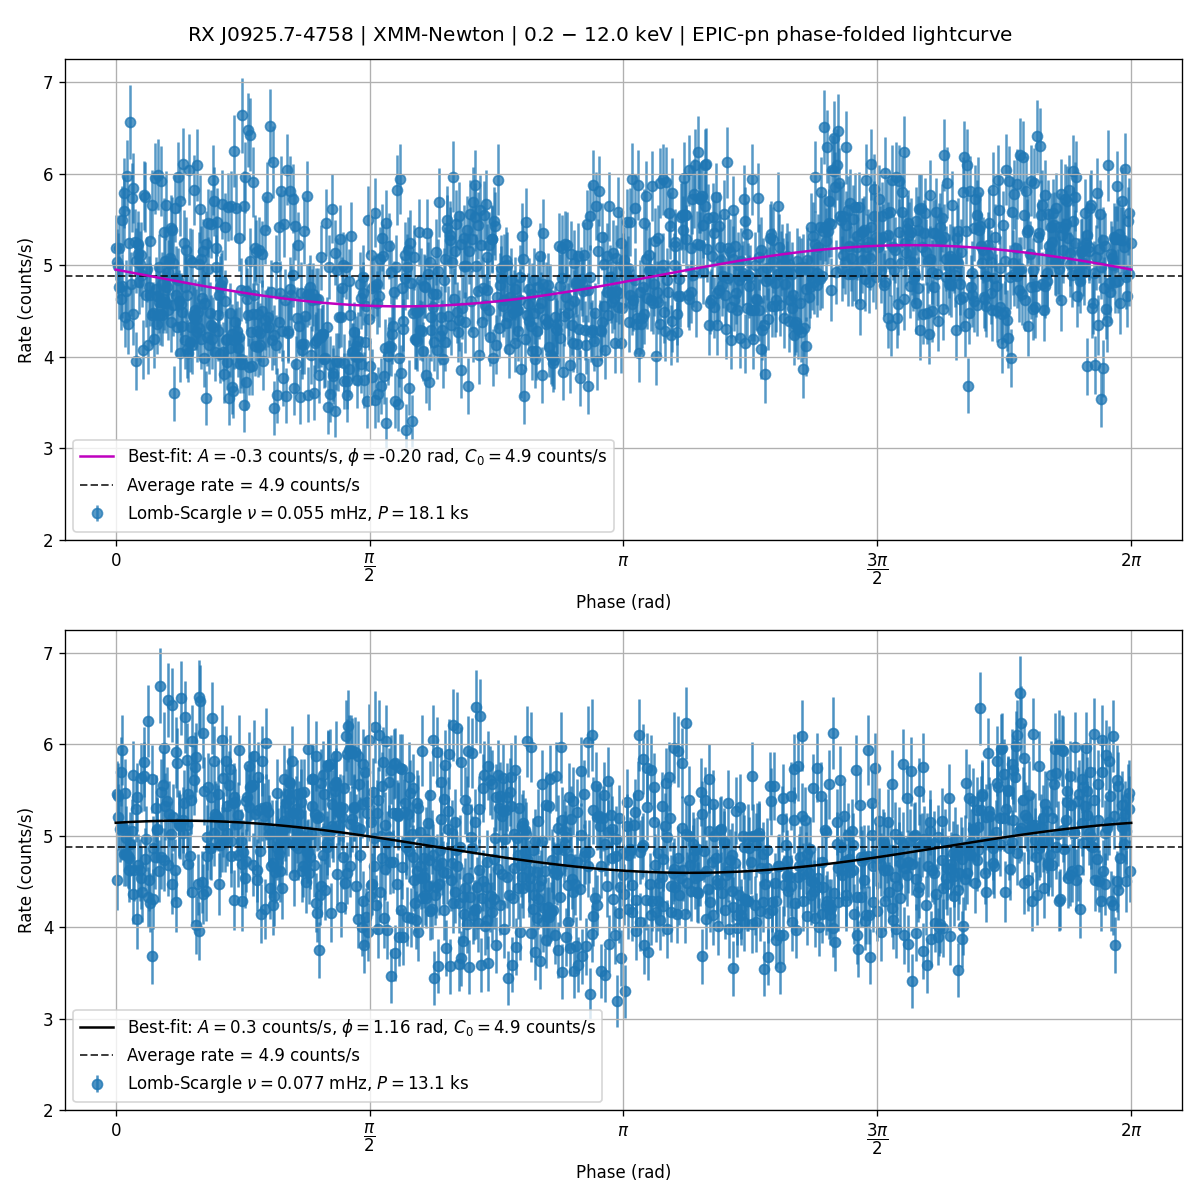
\includegraphics[width=\textwidth]{timing/rx-j0925_0111150101_xmm-lc_200-12000_phasefold-bestfit}
					\caption{Phase-folded XMM-Newton EPIC-pn lightcurve over 0.2--12.0 keV with best-fit sinusoids}
					\label{result:lc-phase-fold-mrvel-xmm:200-12000-bestfit}
				\end{figure}
				For the 0.2--12.0 keV photon energy range using the EPIC-pn instrument of the XMM-Newton observatory, sinusoidal fits were also performed at the frequencies of 0.055 mHz and 0.077 mHz. The phase-folded lightcurve, covering a full cycle from 0 to $2\pi$ radians, is depicted in figure \ref{result:lc-phase-fold-mrvel-xmm:200-12000-bestfit}. The overlaid best-fit sinusoids show a strong correlation with the observed data, confirming the presence of periodic modulations in this broader energy band as well.
				
				\paragraph{Fitting with complete lightcurve:}
				\begin{figure}[h!]
					\centering
					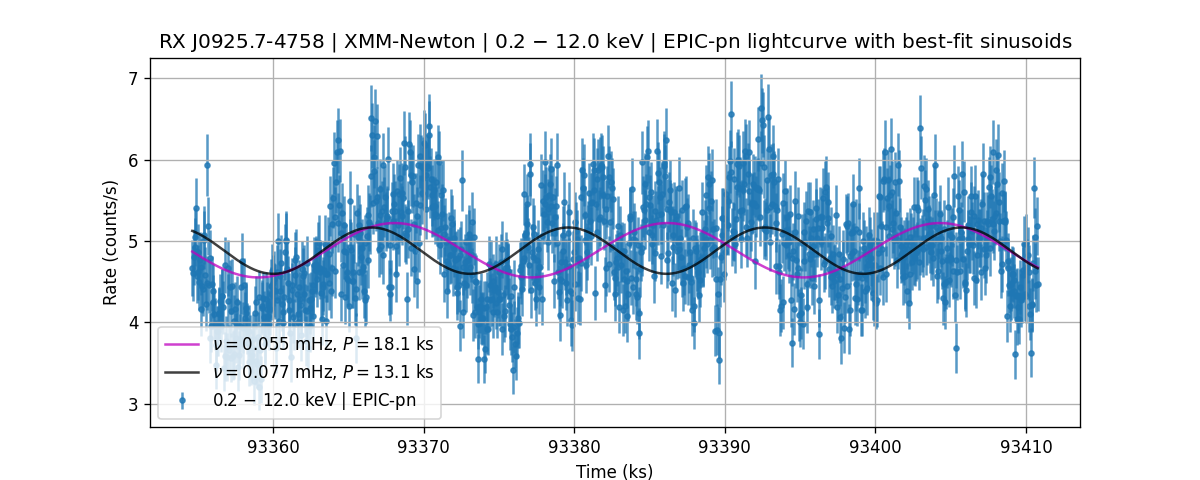
\includegraphics[width=\textwidth]{timing/rx-j0925_0111150101_xmm-lc_200-12000_bestfit}
					\caption{XMM-Newton EPIC-pn lightcurve over 0.2--12.0 keV with best-fit sinusoids}
					\label{result:lc-mrvel-xmm:200-12000-bestfit}
				\end{figure}
				The best-fit sinusoids have been overlaid on the complete lightcurve for the 0.2--12.0 keV photon energy range using the EPIC-pn instrument of the XMM-Newton observatory, as shown in figure \ref{result:lc-mrvel-xmm:200-12000-bestfit}. Here as well, this allows for a visual assessment of how well the sinusoidal models align with the observed data across the entire energy range.
			
			\newpage
			\subsubsection{Best-Fit Sinusoid for 0.2--12.0 keV RGS Lightcurve}
				\paragraph{Fitting with phase-folded lightcurve:}
				\begin{figure}[h!]
					\centering
					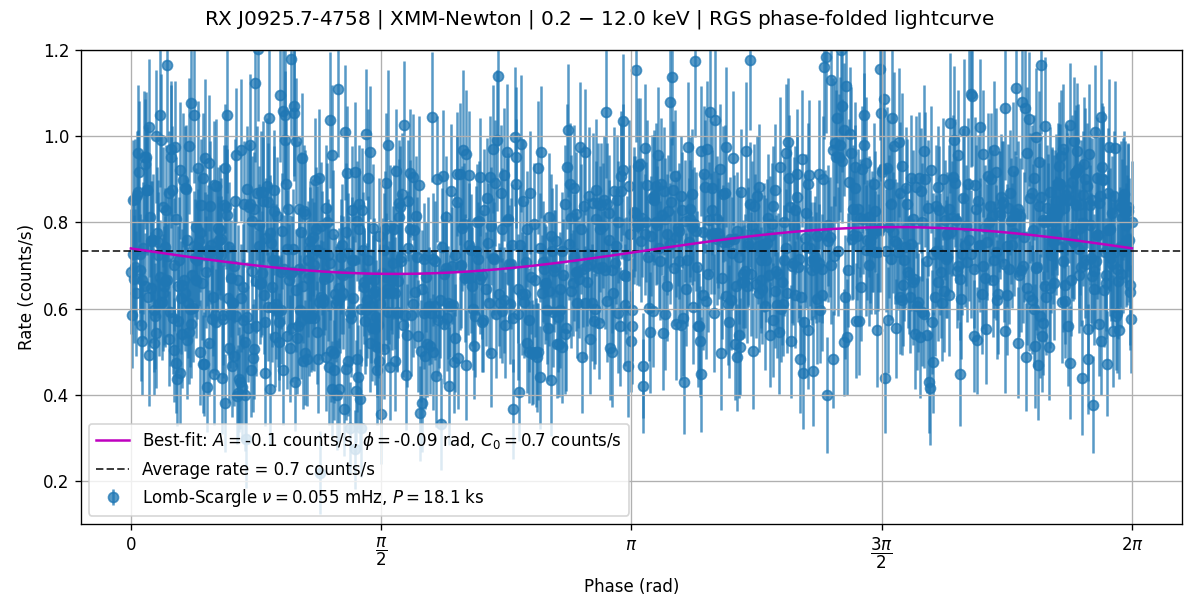
\includegraphics[width=\textwidth]{timing/rx-j0925_0111150101_xmm-rgs-lc_200-12000_phasefold-bestfit}
					\caption{Phase-folded XMM-Newton RGS lightcurve over 0.2--12.0 keV with best-fit sinusoid}
					\label{result:lc-phase-fold-mrvel-xmm-rgs:200-12000-bestfit}
				\end{figure}
				For the 0.2--12.0 keV photon energy range using the RGS instrument of XMM-Newton, sinusoidal fits were applied using only the frequency of 0.055 mHz, as the peak at 0.077 mHz was relatively much weaker (as it can be observed in figure \ref{result:ls-mrvel-xmm}). The resulting phase-folded lightcurve, covering a full cycle from 0 to $2\pi$ radians, is presented in figure \ref{result:lc-phase-fold-mrvel-xmm-rgs:200-12000-bestfit}. The best-fit sinusoid at 0.055 mHz is overlaid on the data, demonstrating a notable correlation with the observed lightcurve.
				
				\paragraph{Fitting with complete lightcurve:}
				\begin{figure}[h!]
					\centering
					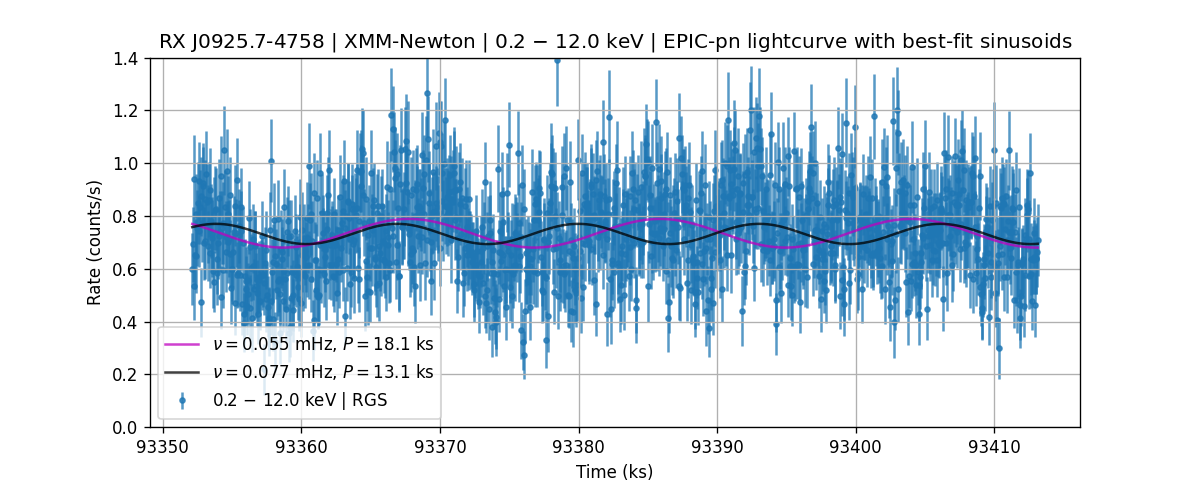
\includegraphics[width=\textwidth]{timing/rx-j0925_0111150101_xmm-rgs-lc_200-12000_bestfit}
					\caption{XMM-Newton RGS lightcurve over 0.2--12.0 keV with best-fit sinusoid}
					\label{result:lc-mrvel-xmm-rgs:200-12000-bestfit}
				\end{figure}
				The best-fit sinusoid for the 0.2--12.0 keV photon energy range from the RGS instrument of XMM-Newton is overlaid on the complete lightcurve, as shown in figure \ref{result:lc-mrvel-xmm-rgs:200-12000-bestfit}. This visualisation enables a direct assessment of how well the sinusoidal model aligns with the observed data across the entire energy range.

		\subsection{Summary of Timing Analysis of \source}
		Table \ref{tab:timing-mrvel} summarizes the timing analysis results for \source\ based on NICER and XMM-Newton light curves. Lomb-Scargle periodograms were employed to identify significant periodicities, with corresponding peak frequencies, periods, and power densities tabulated.
		
		In order to characterize the sinusoidal modulation, phase-folded light curves were fitted with a simple sinusoid model. The derived parameters include amplitude ($A$), average signal level ($C_0$), and initial phase ($\phi$). Additionally, an \textit{amplitude-to-mean ratio} (AMR) was calculated as a percentage, quantifying the variability strength relative to the mean signal level. AMR provides a valuable metric for assessing the significance of the observed periodic behavior.
		\begin{landscape}
		\renewcommand{\arraystretch}{1.5}
		\begin{table}[!htb]
			\centering
			\caption{Results of variability studies on \source}
			\label{tab:timing-mrvel}
			\begin{tabular}{C{2.2cm}C{1.8cm}|C{2cm}C{2cm}C{2cm}C{2cm}|C{1.8cm}C{1.4cm}C{1.8cm}C{1.4cm}}
				\hline
				\multirow{2}{*}{\shortstack{\textbf{Observatory}\\ \textbf{and}\\ \textbf{Instrument}}} & \multirow{2}{*}{\shortstack{\textbf{Photon}\\ \textbf{energy}\\ \textbf{range}}} & \multicolumn{4}{c|}{\textbf{Lomb-Scargle periodogram}} & \multicolumn{4}{c}{\textbf{Best-fit sinusoid}} \\ \cline{3-10}
				{} & {} & {\textbf{Freq. (mHz)}} & {\shortstack{\textbf{Period}\\ \textbf{(ks)}}} & {\textbf{L-S power}} & {\textbf{FAP}} & {\shortstack{$\boldsymbol{A}$\\ \textbf{(counts/s)}}} & {\shortstack{ $\boldsymbol{\phi}$\\ \textbf{(rad)}}} & {\shortstack{$\boldsymbol{C_0}$\\ \textbf{(counts/s)}}} & {\textbf{AMR}} \\
				\hline
				\multirow{4}{*}{\shortstack{NICER\\ \\ XTI}} & \multirow{2}{*}{\shortstack{0.2 -- 1.0\\ keV}} & {0.009} & {112.3} & {0.480} & {$3.9\times 10^{-25}$} & {1.56} & {0.50} & {10.32} & {15.1\%} \\
				{} & {} & {0.017} & {58.8} & {0.490} & {$6.1\times 10^{-26}$} & {1.25} & {1.57} & {10.39} & {12.0\%} \\
				\cline{2-10}
				{} & \multirow{2}{*}{\shortstack{0.2 -- 12.0\\ keV}} & {0.009} & {112.3} & {0.322} & {$1.2\times 10^{-90}$} & {1.76} & {0.48} & {11.63} & {15.1\%} \\
				{} & {} & {0.017} & {58.8} & {0.293} & {$1.2\times 10^{-90}$} & {1.29} & {1.44} & {11.75} & {11.0\%} \\
				\hline
				\multirow{4}{*}{\shortstack{XMM-\\Newton \\ \\ EPIC-pn}} & \multirow{2}{*}{\shortstack{0.2 -- 1.0\\ keV}} & {0.055} & {18.1} & {0.157} & {$7.1\times 10^{-38}$} & {0.31} & {-0.20} & {4.62} & {6.7\%} \\
				{} & {} & {0.077} & {13.1} & {0.095} & {$4.3\times 10^{-23}$} & {0.25} & {1.12} & {4.61} & {5.4\%} \\
				\cline{2-10}
				{} & \multirow{2}{*}{\shortstack{0.2 -- 12.0\\ keV}} & {0.055} & {18.1} & {0.160} & {$8.9\times 10^{-21}$} & {0.33} & {-0.20} & {4.89} & {6.8\%} \\
				{} & {} & {0.077} & {13.1} & {0.106} & {$1.2\times 10^{-18}$} & {0.28} & {1.16} & {4.88} & {5.8\%} \\
				\hline
				{XMM-Newton RGS} & {0.2 -- 12.0 keV} & {0.055} & {18.1} & {0.057} & {$7.3\times 10^{-12}$} & {0.05} & {-0.09} & {0.73} & {7.4\%} \\
				\hline
			\end{tabular}
		\end{table}
		\renewcommand{\arraystretch}{2.2}
		\end{landscape}

	\setcounter{footnotecount}{\value{footnote}}